\documentclass[tikz,border=2pt]{standalone}
\renewcommand{\familydefault}{\sfdefault}
\usetikzlibrary{arrows.meta,calc,positioning}
\tikzset{every picture/.style={line width=1pt, >=Stealth},
         hl/.style={fill=black, fill opacity=0.12, text opacity=1}}
\begin{document}
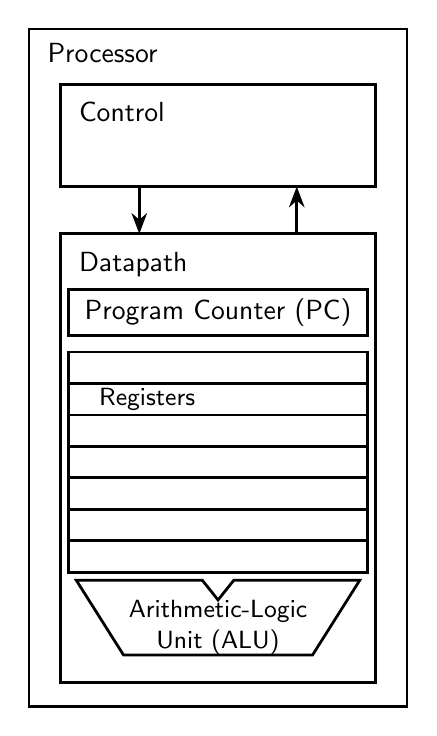
\begin{tikzpicture}[box/.style={draw, minimum width=3.8cm}]
  \draw (0, 0) rectangle (4.8, -8.6);
  \node[anchor=north west] at (0.1, -0.05) {Processor};
  \draw (0.4, -0.7) rectangle (4.4, -2) node[pos=0, below right] {};
  \node[anchor=north west] at (0.5, -0.8) {Control};
  \draw[->] (1.4, -2) -- (1.4, -2.6);
  \draw[<-] (3.4, -2) -- (3.4, -2.6);
  \draw (0.4, -2.6) rectangle (4.4, -8.3);
  \node[anchor=north west] at (0.5, -2.7) {Datapath};
  \node[box, minimum height=0.5cm] at (2.4, -3.6) {Program Counter (PC)};
  \foreach \k in {0, ..., 6} \draw (0.5, -4.1 - 0.4*\k) rectangle (4.3, -4.5 - 0.4*\k);
  \node[fill=white, fill opacity=0, text opacity=1, font=\small] at (1.5, -4.7) {Registers};
  % The ALU symbol: a trapezoid with a notch where its two inputs enter.
  \draw (0.6, -7) -- (2.2, -7) -- (2.4, -7.25) -- (2.6, -7) -- (4.2, -7) -- (3.6, -7.95) -- (1.2, -7.95) -- cycle;
  \node[align=center, font=\small] at (2.4, -7.6) {Arithmetic-Logic \\ Unit (ALU)};
\end{tikzpicture}
\end{document}
